	\section{Test}
	
	\subsection{Unit Test}
	There are parallel with code development been written tests to see if the code reacted as intended. \\
	
	\noindent Jonas and Cecilie chose to use TDD to the development of their code, so there are tests written before the code itself was written, to ensure that all code was covered by the test from the start. \\
	
	\noindent Ao and Morten decided to develop code first, then write their test . This was the choice as there were some difficulties with TDD for them. It worked fine. However, this probably took a little longer than if you had used TDD, as there were some areas of the code you forgot to get tested at the start \\
	
	
	\subsection{Integrations Test}
	Integration testing is used to ensure that all our classes work together, after we have been in two teams and made ​code to the ATM. \\
	Below are our dependency tree for our ATM system
	
	\begin{figure} [!ht]
		\begin{center}
			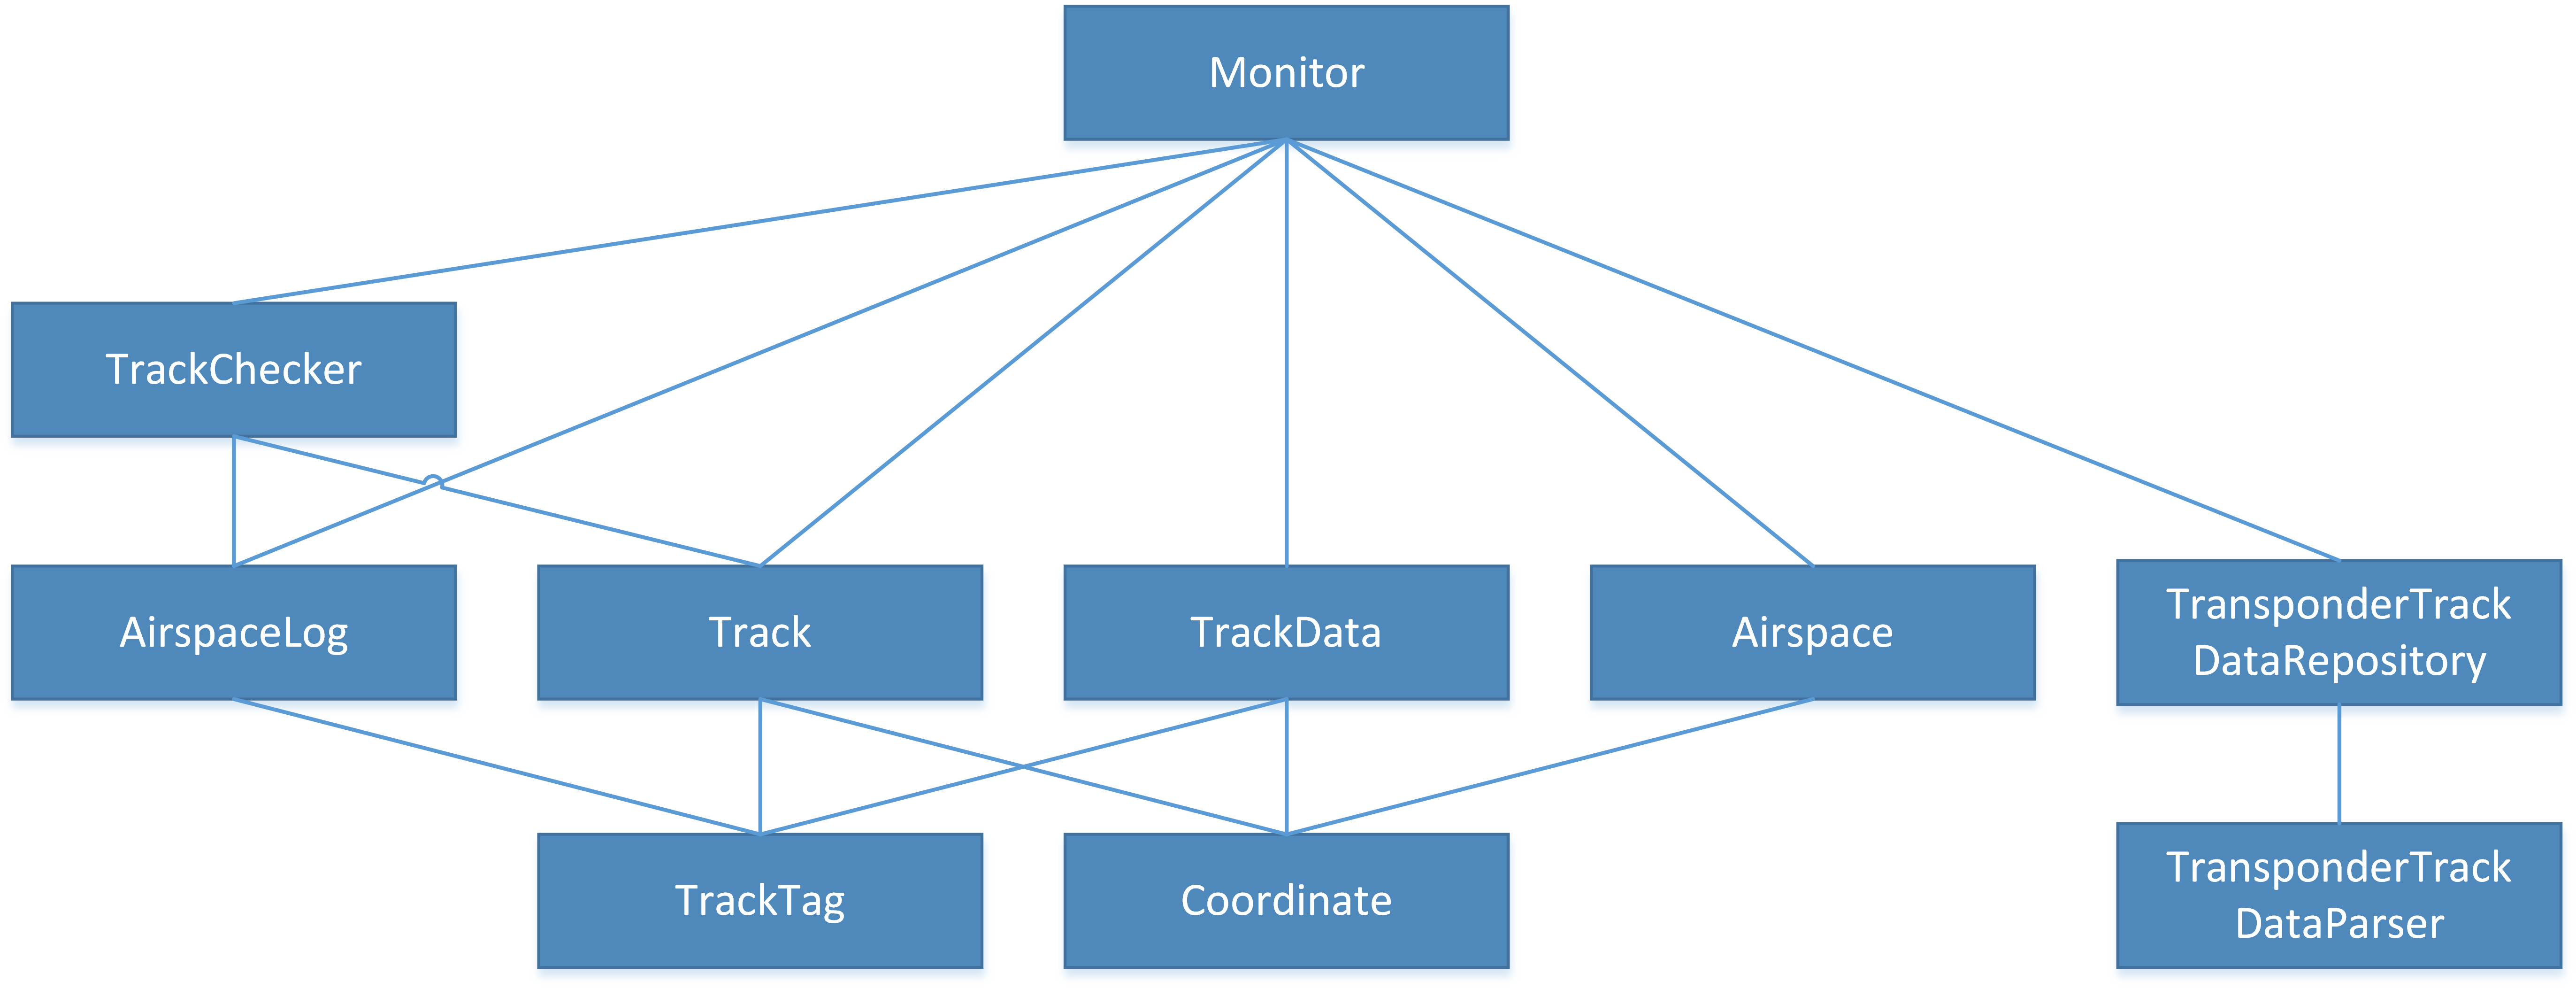
\includegraphics[height=10cm, width=11cm]{Images/Dependencytree}
		\end{center}
		\caption{Dependency Tree for ATM}
		\label{fig:DependencyTree}
	\end{figure}
	\pagebreak
	
	\noindent After making all of our unit tests we designed a dependency tree to find out how we should write our integration test. The Dependency tree shows the integration and interdependence of our different classes. We have chosen to use a bottom-up integration. The choice behind this is that a lot of our test and integration test lies in our unit test. Therefore, all the lower classes is tested and work properly before being coupled to a different class.
	
	\subsection{Jenkins}
	There has previously been described how CI fungrerer as a group tool. \\
	The way we have chosen to use it is via Jenkins, a program that ensures CI on our repository. When comiting code to the repository  Jenkins will first run a build that looks at all the unit tests, if this goes well, Jenkins will subsequent run a project that tests all integration test, once approved it will finally run a project that looks at our code metrics.